\documentclass{article}

% ---------------------------------------------------------------------------
% STA5001 Bayesian & Computational Statistics - Midterm Project Report
% Official NeurIPS 2026 LaTeX template (course-mandated, single column).
% This public copy keeps author names and affiliation and uses placeholders for
% student IDs and school email addresses.
% ---------------------------------------------------------------------------

\usepackage[main, final]{neurips_2026}

\usepackage[utf8]{inputenc}
\usepackage[T1]{fontenc}
\usepackage{hyperref}
\usepackage{url}
\usepackage{booktabs}
\usepackage{amsfonts}
\usepackage{amsmath}
\usepackage{amssymb}
\usepackage{microtype}
\usepackage{xcolor}
\usepackage{graphicx}

% Clean hyperlinks: colour the links and suppress the border boxes that the
% stock template draws around every citation. No style-file setting, margin,
% font or spacing is touched.
\hypersetup{
  colorlinks=true,
  linkcolor=[rgb]{0.00,0.08,0.45},
  citecolor=[rgb]{0.00,0.08,0.45},
  urlcolor=[rgb]{0.00,0.08,0.45},
  pdfborder={0 0 0},
  breaklinks=true,
  bookmarksnumbered=true,
  pdftitle={Weather sensitivity of bike-share usage: a hierarchical Bayesian plan for 25 cities},
  pdfauthor={XUE Yantong, WANG Ziyu, and ZHAO Jiashen},
  pdfsubject={STA5001 Midterm Project},
}

\graphicspath{{../figures/}}

\title{Weather sensitivity of bike-share usage:\\ a hierarchical Bayesian plan for 25 cities}

\author{%
  XUE Yantong \\
  Student ID: 00000000 \\
  Email: student1@example.com \\
  School of Data Science, CUHK-Shenzhen
  \And
  WANG Ziyu \\
  Student ID: 00000000 \\
  Email: student2@example.com \\
  School of Data Science, CUHK-Shenzhen
  \And
  ZHAO Jiashen \\
  Student ID: 00000000 \\
  Email: student3@example.com \\
  School of Data Science, CUHK-Shenzhen
}

\begin{document}

\maketitle

\begin{abstract}
Weather is one of the few influences on bike-share usage that an operator cannot
control.
We assemble a reproducible daily panel from the public release behind
\citet{bean2021weather}: 29 dock-based systems with 8{,}760 hourly records each,
reduced to 10{,}578 city-days. The primary analysis keeps the 25 systems that
record hires on at least 99\% of their analysis days, giving 9{,}120 city-days.
Median daily hires span 6{,}618-fold across these cities, motivating city-specific
usage levels. Each city supplies about one year of data, and a hierarchy will
jointly estimate weather associations and their between-city variation. Binned
within-city averages show a thermal response
peaking near $27.5^\circ$C and then falling, and a rainfall response that
declines monotonically to about $41\%$ below the dry-day bin. We close with the
hierarchical Student-$t$ regression and inference plan for the final project.
\end{abstract}

% ===========================================================================
\section{Introduction}
% ===========================================================================

Bike-share operators allocate bicycles and plan maintenance around changes in
daily use. Thermal comfort and rainfall are relevant to these decisions, but
their associations with use may differ across cities with different climates
and travel patterns.

The reference study \citep{bean2021weather} compares forty cities across climate
zones. It fits a frequentist generalized additive model to each city separately
and reports two robust patterns: hires rise with the Universal Thermal Climate
Index (UTCI) up to roughly $27$--$28^\circ$C and then decline, and rainfall is
associated with lower use. Our question is how to estimate the distribution of
city weather associations jointly, allowing cities to share information while
retaining their own coefficients. Each city supplies about one year of daily
observations. The uncertainty in its weather response therefore matters alongside
the differences between cities. Median daily hires range from $11.5$ in
Cr{\'e}teil to $76{,}103$ in Paris, which motivates separate city intercepts.

We therefore recast the comparison as a hierarchy. Each city keeps its own
intercept, weather coefficients, weekend coefficient and seasonal coefficients,
but those city parameters share a normal population distribution. This answers
three questions that the midterm is designed to set up.

\begin{quote}
\textbf{Research questions.} (1)~How does thermal comfort relative to the local
study-period average relate to daily hires? (2)~How much do cities differ in
their rainfall response? (3)~Are a city's thermal and rainfall background
associated with part of that between-city variation?
\end{quote}

This report documents the data, the cleaning decisions and the exploratory
evidence, and states the model the final project will fit. All statements
describe statistical association; the data cannot identify a causal effect.

% ===========================================================================
\section{Data}
\label{sec:data}
% ===========================================================================

\paragraph{Source and scope.} The data are the public release accompanying
\citet{bean2021weather}, distributed through Mendeley Data
\citep{mendeley2021bikeshare} under CC BY 4.0 (DOI
\texttt{10.17632/2nxpvtz935.1}, Version 1). Hourly hires are estimated from
per-minute station inventory snapshots, may include rebalancing moves and may
carry a $0.5$ fractional part. UTCI combines air temperature, humidity, wind and
radiation to describe thermal stress. UTCI and precipitation come from the
Copernicus Climate Data Store. The archive
carries metadata and weather arrays for forty cities but hourly stock data for
thirty; the paper's R code designates metadata rows 7--34 and row 36 as the 29
dock-based systems, and we keep that scope. Archive and paper
are stored with SHA-256 digests re-checked on every run.

\paragraph{Hourly to daily.} Each city contributes exactly 8{,}760 stock rows.
The source file contains three repeated city--date--hour keys: Brisbane and
Dublin on 2017-10-29 at 02:00, and Melbourne on 2017-04-02 at 02:00. The Dublin
and Melbourne dates coincide with daylight-saving transitions, whereas Brisbane
does not observe daylight saving, so the cause of its duplicate is left
unspecified. Following the paper's rule we preserve row
order and map the 8{,}760 rows onto consecutive UTC hours from the first source
date rather than merging the repeated labels. The hourly series is then converted
to each city's local time zone and aggregated by local date: hires and
precipitation are summed, UTCI contributes its daily mean, minimum and maximum. A
local day enters the analysis only if it lies inside the city's nominal study
period, contains 23 to 25 hourly rows, has at least 20 valid UTCI hours, and has
complete precipitation. Of 10{,}613 candidate city-days, 35 fail at least one
rule, leaving 10{,}578; the reasons overlap: 28 lie outside the nominal period,
34 outside the 23--25 hour count and 33 fall short of 20 UTCI hours.

\paragraph{Primary sample.} Of the 575 zero-hire days in the full panel, 571 sit
in G{\"o}teborg, Kazan, Lillestr{\o}m and Vilnius; long zero runs can reflect
seasonal operation, station recording state or genuinely no use, and the three
are not separable. We therefore restrict the primary analysis in advance to
cities recording hires on at least 99\% of their analysis days, keeping 25 cities
and 9{,}120 city-days and leaving four zero-hire days. The full 29-city panel is
retained in the same file behind a \texttt{continuous\_system} flag. The
processed panel has no missing cells, no negative values and a unique
city--date key; re-running the preparation script reproduces it byte-for-byte.
Table~\ref{tab:audit} summarises the panel.

\begin{table}[t]
  \centering
  \caption{Frozen daily panel and primary sample. The full 29-city panel is
  retained with an indicator identifying the 25-city primary sample.}
  \label{tab:audit}
  \footnotesize
  \begin{tabular}{lrlr}
    \toprule
    \textbf{Item} & \textbf{Value} & \textbf{Item} & \textbf{Value} \\
    \midrule
    Dock-based cities          & 29              & Primary cities          & 25 \\
    Hourly records             & 254{,}040       & Primary city-days       & 9{,}120 \\
    City-days after filtering  & 10{,}578        & Zero-hire days, primary & 4 \\
    Date range                 & 2016-07 -- 2017-12 & Dry-day share        & 21.5\% \\
    Countries or regions       & 10              & Trewartha codes         & 6 \\
    \bottomrule
  \end{tabular}
\end{table}

% ===========================================================================
\section{Exploratory analysis}
\label{sec:eda}
% ===========================================================================

Everything below is computed from the frozen panel with no model and no
imputation. Averages are taken inside cities first and then across cities, so a
single large system cannot dominate a curve.

\paragraph{City scale.} Figure~\ref{fig:overview}a orders the 25 primary cities
by median daily hires, a 6{,}618-fold spread. Figure~\ref{fig:overview}b shows
the continuous-system rule: the four excluded cities record positive hires on
between 35\% and 92\% of analysis days, while every primary city sits above 99\%.

\begin{figure}[t]
  \centering
  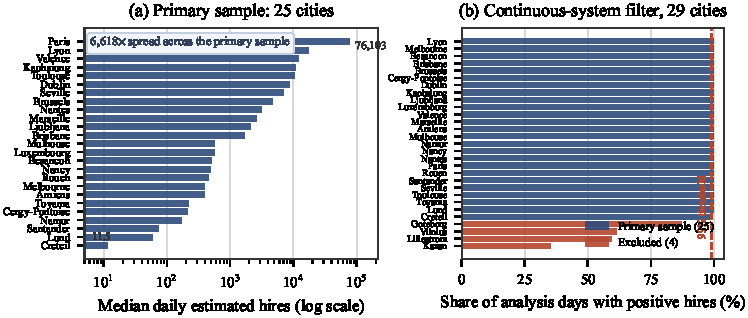
\includegraphics[width=0.85\textwidth]{report_fig1_data_overview.pdf}
  \caption{(a) Median daily hires for the 25 primary cities on a log scale.
  (b) Share of analysis days with positive hires for all 29 dock-based cities,
  with the 99\% inclusion threshold.}
  \label{fig:overview}
\end{figure}

\paragraph{Thermal response.} Figure~\ref{fig:response}a bins city-days by daily
mean UTCI in $5^\circ$C intervals and plots within-city centred
$\log(1+\text{hires})$ against the bin centre, with the 25th to 75th percentile
band across cities. The curve reaches its global maximum of $+0.26$ near
$27.5^\circ$C, against $-0.26$ in the coldest populated bin ($-22.5^\circ$C) and
$-0.14$ in the hottest bin ($32.5^\circ$C); the three coldest bins are not
ordered monotonically. The peak agrees with the $27$--$28^\circ$C of
\citet{bean2021weather}, and the drop to the hottest bin is $0.41$ log units. The
band across cities is $0.38$ log units wide at the peak, which is the
between-city variation that questions~(2) and~(3) target.

\paragraph{Rainfall response.} Figure~\ref{fig:response}b bins city-days by daily
precipitation. The dry bin sits $+0.16$ above the city mean and the response
declines monotonically across the six bins, reaching $-0.36$ above 20\,mm, which
is $0.52$ log units and about $41\%$ below the dry bin on the hires scale. That
contrast is descriptive: it compares two bins of the pooled curve with no
adjustment for season, city or the other covariates. Rainfall has a consistent
sign, but the figure shows only the pooled shape; how much it varies across
cities is what the hierarchical model will estimate.

\begin{figure}[t]
  \centering
  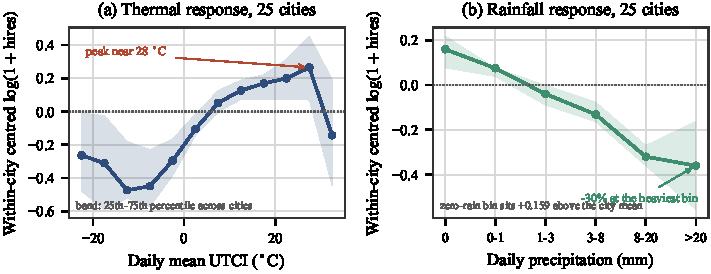
\includegraphics[width=0.85\textwidth]{report_fig2_weather_usage.pdf}
  \caption{Within-city centred $\log(1+\text{hires})$ against (a) daily mean UTCI
  and (b) daily precipitation, for the 25 primary cities. Points are city-equal
  bin averages; the shaded band spans the 25th to 75th percentile across cities.}
  \label{fig:response}
\end{figure}

\paragraph{Season and week.} Figure~\ref{fig:season}a shows the seasonal profile,
peaking in mid-October and troughing at the end of December with a descriptive
range of $0.84$ log units.
Figure~\ref{fig:season}b ranks cities by the weekend-minus-weekday difference:
23 of 25 are negative, with a mean of $-0.55$, and Melbourne is the only clearly
positive city at $+0.27$.

\begin{figure}[t]
  \centering
  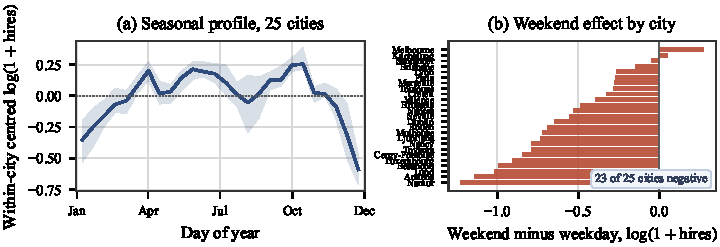
\includegraphics[width=0.85\textwidth]{report_fig3_seasonality.pdf}
  \caption{(a) Seasonal profile of within-city centred $\log(1+\text{hires})$ by
  day of year, with the same percentile band as Figure~\ref{fig:response}.
  (b) Weekend-minus-weekday difference for each primary city, sorted.}
  \label{fig:season}
\end{figure}

\paragraph{Implications for the specification.} The thermal curve motivates a
nonlinear term; we use a quadratic as a compact representation. Variation across
cities motivates city-specific coefficients with a shared distribution. The
seasonal profile motivates adjustment for the annual cycle when estimating
weather associations. Within
cities the annual sine and cosine alone explain $62$--$92\%$ of the variance of
daily UTCI, $76\%$ on average, so they enter as controls and the thermal
coefficient is read with them in the model.
Figure~\ref{fig:response} pools absolute UTCI across cities, whereas the model
targets within-city deviations from each city's own mean conditional on
seasonality, so the descriptive peak motivates a nonlinear thermal term rather
than estimating an optimum temperature.

% ===========================================================================
\section{Plan for the final project}
\label{sec:plan}
% ===========================================================================

\paragraph{Model.} Let $U_{it}$ be estimated hires for city $i$ on local day $t$
and $y_{it}=\log(1+U_{it})$. The response follows a Student-$t$ observation
distribution,
\[
  y_{it}\sim t_{\nu}\!\left(\mu_{it},\sigma_i\right),
  \qquad
  \mu_{it}=\alpha_i+\beta_{1i}T_{it}+\beta_{2i}Q_{it}+\beta_{3i}R_{it}
  +\beta_{4i}W_{it}+\beta_{5i}S_{it}+\beta_{6i}C_{it},
\]
where $T_{it}$ is the training-centred daily UTCI in $10^\circ$C units,
$Q_{it}$ its training-centred square, and $R_{it}$ training-centred
$\log(1+\text{mm})$ divided by the pooled within-city training standard deviation.
$W_{it}$ indicates weekends; $S_{it}$ and $C_{it}$ are the annual sine and cosine
of $2\pi d_{it}/365.25$. Student-$t$ accommodates extreme days. City coefficients
share normal population distributions, whose weather centres vary with city
thermal and rainfall backgrounds to address question~(3).

\paragraph{Priors and computation.} Normal priors on population coefficients and
HalfNormal priors on between-city scales regularise the weather response on the
$\log(1+U)$ scale. We use $\nu=2+\text{Exponential}(0.1)$ to allow heavy tails with
finite variance. NUTS through PyMC \citep{abrilpla2023pymc} and nutpie
\citep{nutpie} will estimate the posterior. The accompanying model configuration
specifies the numerical prior scales.

\paragraph{Questions and assessment.} Posterior contrasts will quantify weather
associations, city variation and background associations. A predictive extension
will compare calendar and residual time
structures on eight-week holdouts, using interval scores, coverage and point
errors. All preprocessing will use training observations. Checks cover
$\widehat{R}\le1.01$ \citep{vehtari2021rank}, bulk and tail ESS $\ge400$, Monte
Carlo error, divergences, prior and posterior prediction, and residuals
\citep{gabry2019visualization}. Weather prior scales of $0.5$, $1$ and $2$ times
the baseline define the sensitivity comparison. Broader city coverage and
alternative likelihood or seasonal specifications are possible extensions.

\paragraph{Scope.} Each city contributes about one year, so background variables
describe the study period. Hires are inventory-change estimates that may include
rebalancing moves; system size, pricing and operating policy are unobserved.
Conclusions are limited to the 25 continuous dock-based systems.

% ===========================================================================
\section*{Contribution statement}
% ===========================================================================

XUE Yantong searched for data, selected the topic, designed the experiments, developed code,
conducted the analysis, and prepared the report and presentation. WANG Ziyu and ZHAO Jiashen
contributed to data processing, code development and
checking, and verification of the report and slides.

\small
\bibliographystyle{plainnat}
\bibliography{references}

\end{document}
